
\section{GitLab} 
Gitlab es un servicio web de control de versiones y desarrollo de software colaborativo basado en Git. Además de gestor de repositorios, el servicio ofrece también alojamiento de wikis y un sistema de seguimiento de errores, todo ello publicado bajo una Licencia de código abierto.
Fue escrito por los programadores ucranianos Dmitriy Zaporozhets y Valery Sizov en el lenguaje de programación Ruby. La compañía, GitLab Inc., cuenta con un equipo de 150 miembros1​ y más de 1400 usuarios.2​ Es usado por organizaciones como la NASA, el CERN, IBM o Sony.
\begin{itemize}
	\begin{center}
	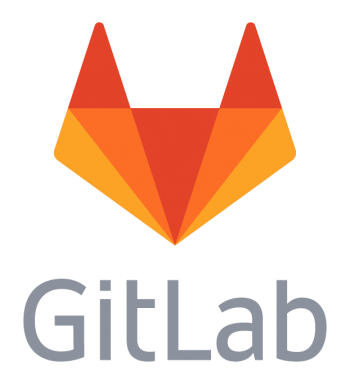
\includegraphics[width=5cm]{./Imagenes/imagen6} 
	\end{center}
\end{itemize} 
Como comentan en The Next Web, GitLab es como GitHub pero en esteroides. Es un servicio que también ofrece alojamiento de repositorios con varias funciones de seguimientos de problemas, pero además tiene características extra.

GitLab fue fundado en 2011, y como cuentan ellos mismos, inició como un proyecto en GitHub. A diferencia de este último, en GitLab usan una aplicación única creada desde cero para dar soporte al ciclo entero de desarrollo, en lugar de integrar múltiples herramientas diferentes.\\



\section{GitLab no es un simple clon de GitHub} \\

También tiene un plan básico gratuito que permite aprovechar la plataforma para construir y ejecutar tus aplicaciones. Y, están aprovechando este momento para ofrecer 75% de descuento en sus planes Gold y Ultimate a los nuevos usuarios.

GitLab tampoco es ningún desconocido, múltiples empresas y marcas conocidas lo usan. Y recientemente el proyecto GNOME se mudó a la plataforma justamente porque buscaban simplificar el proceso de colaboración entre sus múltiples contribuidores. La misma gente de GNOME explica que GitLab no es un simple clon de GitHub.